
\begin{figure}
    \centering
    \begin{subfigure}[b]{0.3\textwidth}
        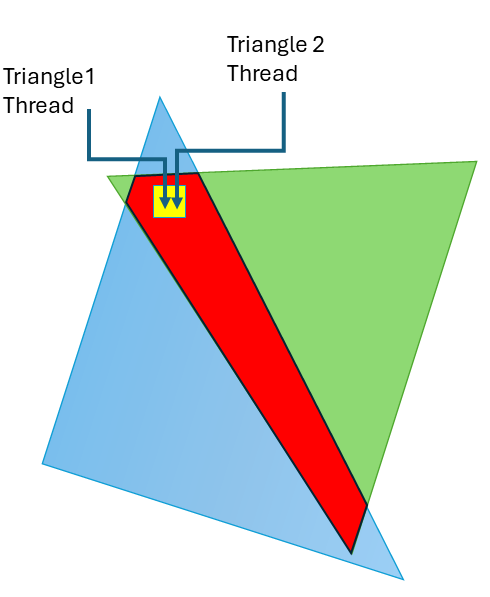
\includegraphics[width=\textwidth]{TriangleJoinsA}
		 \subcaption[short for lof]{A}
        \label{fig:gull}
    \end{subfigure}
    ~ %add desired spacing between images, e. g. ~, \quad, \qquad, \hfill etc. 
      %(or a blank line to force the subfigure onto a new line)
    \begin{subfigure}[b]{0.3\textwidth}
        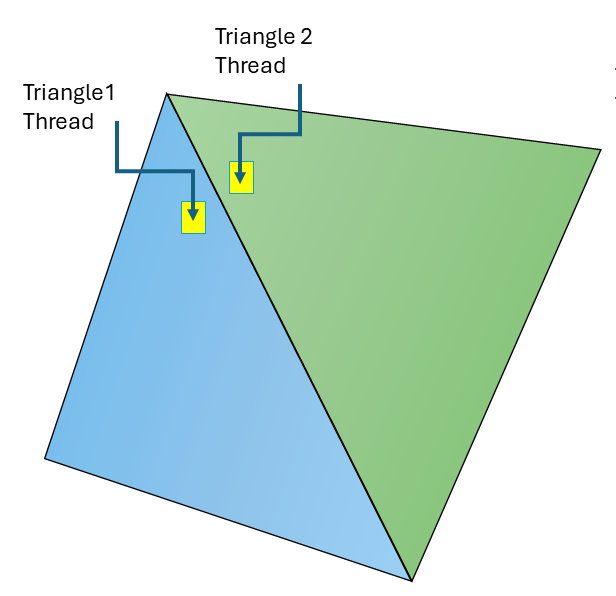
\includegraphics[width=\textwidth]{TriangleJoinsB}
 		\subcaption[short for lof]{B}
        \label{fig:tiger}
    \end{subfigure}
  \captionof{figure}[TITLE:Plot of fps v loadedp]{\textit{No Caption}}
\end{figure}